\section{Композиция и суперпозиция. Замкнутые множества функций}

Для задания функций в виде формул чаще всего используют так называемые
элементарные функции, которые строятся по правилам образования сложных
функций с помощью системы
\begin{equation}\tag{1.9}
\begin{gathered}
H_\varepsilon=\Bigl\{x\pm y;\ xy;\ \frac xy;\ x^n;\ a^x\ (a>0);\ \log_ax\ (a>0);\\
\sin x;\ \cos x;\ \tg x;\ \ctg x;\ \arcsin x;\ \arccos x;\ \arctg x;\\
\operatorname{arcctg}x;\ a,\ \forall a\in\R\Bigr\},
\end{gathered}
\end{equation}
состоящей из арифметических операций, основных элементарных функций
и констант.

Примерами элементарных функций являются $e^{2\sin^2xy}$;
$\dfrac{x_1x_2+\arctg x_3}{1+x_1x_2x_3}$; $(2(x_1x_2+x_3)+x_4)+2$;
$\sqrt{t^2}$ и~др. Последняя из них $\sqrt{t^2}=|t|$ ($t$ "---
действительная переменная), если ее умело использовать, позволяет считать
элементарными и многие кусочно-элементарные функции (но не все, если речь
идет о функциях более чем одного аргумента!), т.\,е. функции, задаваемые
различными элементарными формулами в различных подобластях пространства
аргументов. Например, можно убедиться, что функция
\begin{equation}\tag{1.10}
h_1(x)=\begin{cases}0&\text{при }|x|>1;\\ 1+x&\text{при }-1\le x\le0;\\ 1-x&\text{при }0<x\le1\end{cases}
\end{equation}
может быть также задана одной формулой:
\[
h_1(x)=\tfrac12\bigl(1-|x|+|1-|x||\bigr).
\]
(График функции $h_1(x)$ показан на рис.~8.)

\begin{figure}[h]
\centering
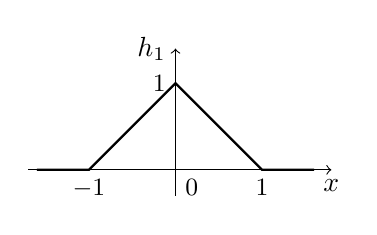
\begin{tikzpicture}[scale=1.1]
 \draw[->] (-1.7,0)--(1.8,0) node[below]{$x$};
 \draw[->] (0,-0.3)--(0,1.4) node[left]{$h_1$};
 \draw[thick] (-1.6,0)--(-1,0)--(0,1)--(1,0)--(1.6,0);
 \node[below] at (-1,0){\small $-1$}; \node[below] at (1,0){\small 1};
 \node[below right] at (0,0){\small 0}; \node[left] at (0,1){\small 1};
\end{tikzpicture}
\figcap{Рис. 8.}
\end{figure}

Во времена Ньютона и Лейбница понятие функции по существу исчерпывалось
элементарными функциями. Лишь позже, когда было установлено, что некоторые
интегралы от элементарных функций нельзя представить в элементарном виде,
не все уравнения с элементарными коэффициентами можно разрешить
в элементарных функциях и так далее, возникла общая
теоретико-множественная
\bookpage{23}%
точка зрения и элементарные функции стали рассматриваться как примеры
функций вообще.

По мере развития математики число функций, для которых вводилась
стандартная символика, постепенно расширялось, причем происходило это
в рамках как элементарных функций (например, гиперболические функции
$\operatorname{sh}x$, $\operatorname{ch}x$, $\operatorname{th}x$ и~др.),
так и специальных функций (Эйлера, Бесселя, Матье и~т.\,д.). Заметим, что
расширение символики осуществлялось путем своего рода <<естественного
отбора>> и определялось прежде всего практической значимостью
рассматриваемых функций.

Необходимость совершенствования конструктивных средств математики, которые
до недавнего времени почти исчерпывались базисной системой (1.9), особенно
возросла в последние годы, когда широкое распространение получили
быстродействующие вычислительные машины и возникла проблема повышения
эффективности их использования. В частности, появились серьезные основания
для расширения системы (1.9) как в рамках самих элементарных функций, так
и за их пределами.

В дальнейшем наряду с системой (1.9) будут рассматриваться и другие
базисные системы (например, системы булевых функций, $R$-функций и~др.),
поэтому целесообразно подойти к вопросу формирования сложных функций
с помощью базисных систем с общих позиций.

Пусть $\mathfrak X$ "--- некоторое множество, $\mathfrak X^n$ "--- его $n$-я
степень. Отображения вида
$y=f(x)\colon\mathfrak X^n\to\mathfrak X^m$, $x=(x_1,\dots,x_n)$,
$y=(y_1,\dots,y_m)$ назовем \emph{правильными с алфавитом $\mathfrak X$}.
Множество всех правильных с алфавитом $\mathfrak X$ отображений обозначим
$\mathfrak F(\mathfrak X)$. При $m=1$ правильные отображения вида
$f\colon\mathfrak X^n\to\mathfrak X$ называются $n$-местными ($n$-арными)
\emph{алгебраическими операциями} на $\mathfrak X$~[45].

Пусть $y=f(x)\colon\mathfrak X^n\to\mathfrak X^m$;
$u=\varphi(y)\colon\mathfrak X^m\to\mathfrak X^p$. Отображение
$u=\varphi[f(x)]\colon\mathfrak X^n\to\mathfrak X^p$ принято называть
\emph{композицией} $f$ и $\varphi$. Для композиции применяется также
обозначение $\varphi[f(x)]=\varphi\circ f$.

Введем понятие \emph{суперпозиции}, некоторым образом обобщающее понятие
композиции. Пусть $H$ "--- некоторая система (не обязательно конечная)
правильных с алфавитом $\mathfrak X$ отображений
\begin{equation}\tag{1.11}
H=\{y=\varphi_i(x)\colon\mathfrak X^{n_i}\to\mathfrak X^{m_i},\ i\in I_0\},
\end{equation}
где $I_0$ "--- некоторое множество индексов.

Множество $\M(H)$ суперпозиций системы $H$ включает:

а) отображения, составляющие $H$;

б) тождественное отображение $y\equiv x\colon\mathfrak X\to\mathfrak X$;

в) отображения вида
$f=(\varphi,\psi)\colon\mathfrak X^n\to\mathfrak X^{m+p}$, где
$\varphi\colon\mathfrak X^n\to\mathfrak X^m$,
$\psi\colon\mathfrak X^n\to\mathfrak X^p$,
$(\varphi,\psi)=(\varphi_1,\dots,\varphi_m,\psi_1,\dots,\psi_p)$,
а $\varphi,\psi\in\M(H)$;

г) композиции вида $\varphi\circ\psi$, $\varphi,\psi\in\M(H)$.
\bookpage{24}%

Для того чтобы подчеркнуть происхождение суперпозиций от базисной системы
$H$, элементы множества $\M(H)$ будем называть \emph{$H$-реализуемыми
отображениями}, а если $\mathfrak X$ "--- числовое множество, то
\emph{$H$-реализуемыми функциями}.

Понятие $H$-реализуемой функции является формализацией понятия функции,
заданной аналитически (в виде единого аналитического выражения).
Действительно, если для обозначения функций, составляющих базисную систему
(1.11), ввести некоторый набор символов, то для каждой $H$-реализуемой
функции можно будет написать формулу, содержащую лишь указанные символы,
символы независимых переменных и, возможно, открывающие и закрывающие
скобки.

Классическим примером применения операции суперпозиции являются
элементарные функции, которые в соответствии с введенной терминологией
можно назвать $H_\varepsilon$-реализуемыми функциями (с базисной системой
(1.9)).

Заметим, что при образовании суперпозиций (в силу пункта <<б>> их
определения) допускается произвольное переименование независимых
переменных. Так, например, суперпозициями системы
$H=\{f(x_1,x_2,x_3),\ \varphi(x_1,x_2),\ \psi(x_1,x_2)\}$ являются функции
$f[\varphi(x_1,x_2),x_2,\psi(x_3,x_4)]$;
$f[\varphi(x_1,x_2),x_1,f(x_1,x_1,x_1)]$; $\psi[\varphi(x,y),\varphi(u,t)]$.

Рассмотрим наряду с системой
$H=\{y=\varphi_i(x)\colon\mathfrak X^{n_i}\to\mathfrak X^{m_i},\ i\in I_0\}$
систему
$H_1=\{y=\psi_i(x)\colon\mathfrak X^{n_i}\to\mathfrak X^{m_i},\ i\in I_0\}$,
полученную заменой
\begin{equation}\tag{1.12}
\begin{pmatrix}\varphi_1,&\varphi_2,&\dots,&\varphi_s,&\dots\\ \psi_1,&\psi_2,&\dots,&\psi_s,&\dots\end{pmatrix}
\end{equation}
функций $\varphi_i$ на $\psi_i$, $i\in I_0$ соответственно. (При этом
функции $\psi_i$ имеют то же число аргументов, что и функции $\varphi_i$.)

Пусть $f\in\M(H)$ "--- некоторая $H$-реализуемая функция. Ей соответствует
некоторая формула $f[\varphi_{\alpha_1},\dots,\varphi_{\alpha_m}]$,
$\alpha_i\in I_0$,\fixed{в оригинале
$f[\varphi_{\alpha_1},\dots,\varphi_{\alpha_n}]$ при последующем
$\varphi_{\alpha_1},\dots,\varphi_{\alpha_m}$.} в которую входят какие-то
функции $\varphi_{\alpha_1},\dots,\varphi_{\alpha_m}$ из $H$. Заменим в этой
формуле, согласно (1.12), функции $\varphi_i$ на $\psi_i$,\fixed{в оригинале
<<Заменим в формуле (1.12) функции $\varphi_i$ на $\psi_i$>>; (1.12) "--- это
таблица замены, а заменяются функции в формуле для $f$.} сохранив при этом
наименование независимых переменных. В результате получим новую функцию
$f_1\in\M(H_1)$, описываемую формулой
$f[\psi_{\alpha_1},\dots,\psi_{\alpha_m}]$.

Формулы $f[\varphi_{\alpha_1},\dots,\varphi_{\alpha_m}]$
и $f[\psi_{\alpha_1},\dots,\psi_{\alpha_m}]$ называются \emph{формулами
одинаковой структуры}.

Пусть, например, $H=H_\varepsilon$ (1.9), $u=(x_1x_2+3)\,e^{x_1x_2}$, и дана
замена:
\[
\begin{pmatrix}x_1x_2;&x_1+x_2;&e^t;&3\\ x_1+x_2;&x_1x_2;&\sin t;&5\end{pmatrix}.
\]
Тогда формула $v=(x_1+x_2)5+\sin(x_1+x_2)$ имеет ту же структуру, что
и формула $u=(x_1x_2+3)\,e^{x_1x_2}$.

С понятием суперпозиции тесно связано понятие \emph{замкнутого}
множества. Множество $\M_0$ называется \emph{суперпозиционно замкнутым},
если для всякой системы $H\subset\M_0$ множество суперпозиций
$\M(H)\subset\M_0$.
\bookpage{25}%

Если все возможные композиции функций из $\M$ принадлежат $\M$, то
множество $\M$ будем называть \emph{композиционно
замкнутым}.\fixed{в оригинале: <<Если все возможные композиции функций из
$\M$ принадлежат $\M$, но имеются суперпозиции функций из $\M$, не
принадлежащие $\M$, то множество $\M$ будем называть композиционно
замкнутым>>. С оговоркой <<но имеются\dots>> следующая фраза
(<<всякое замкнутое множество является композиционно замкнутым>>) была бы
неверна; оговорка описывает множества, композиционно, но не
суперпозиционно замкнутые.}

В дальнейшем, для сокращения речи, суперпозиционно замкнутые множества
будем называть \emph{замкнутыми}. Очевидно, что всякое замкнутое множество
является композиционно замкнутым.

Примерами замкнутых множеств являются:

1) множество $C^k(\R^n)$ ($n=1,2,\dots$) $k$ раз непрерывно
дифференцируемых везде функций (в том числе множества $C^0=C$ непрерывных
и $C^\infty$ бесконечно дифференцируемых функций);

2) множества $C^R$ целых рациональных функций и $C^Q$ "---
дробно-рациональных функций;

3) множество $C^A$ везде аналитических функций (т.\,е. разложимых в ряд
Тейлора в окрестности любой точки);

4) множество $\mathfrak F(\mathfrak X)$ правильных отображений с непустым
алфавитом $\mathfrak X$;

5) пусть $\M=\mathfrak F(\mathfrak X)$ множество правильных отображений
с алфавитом $\mathfrak X$, а $a\in\mathfrak X$. Рассмотрим множество
$\M_a\subset\M$ всех таких отображений\fixed{в оригинале $T_a$; в конце абзаца это же множество обозначено $\M_a$.}
$f\colon\mathfrak X^n\to\mathfrak X^m$ ($\forall n,m\in\N$), которые
переводят элементы вида $(a,a,\dots,a)\in\mathfrak X^n$ в элементы вида
$(a,a,\dots,a)\in\mathfrak X^m$. В частности, если $\mathfrak X\subset\R$
и $a=0\in\mathfrak X$, то отображения вида $f\colon\mathfrak X^n\to\mathfrak X$,
обладающие отмеченным свойством, принято называть \emph{алгебраическими
операциями, сохраняющими~0}. Для таких операций всегда $f(0,0,\dots,0)=0$.
Нетрудно доказать (это непосредственно видно из определения суперпозиции),
что множество $\M_a$ замкнуто.

\textbf{Теорема 1.} \emph{Пересечение замкнутых (композиционно
замкнутых) множеств есть замкнутое (композиционно замкнутое) множество.
(Пустое множество считается замкнутым по определению.)}

\textsc{Доказательство.} Пусть $\M_1$ и $\M_2$ "--- замкнутые множества,
а $H\subset\M_1\cap\M_2$. Тогда множество $\M(H)$ $H$-реализуемых функций
должно в силу замкнутости $\M_1$ и $\M_2$ содержаться в каждом из них.
Следовательно, $\M(H)\subset\M_1\cap\M_2$, что и требовалось доказать.

В дальнейшем широко используется понятие полной системы отображений, смысл
которого заключается в следующем. Система $H$ называется \emph{полной} по
отношению к множеству $\M_0$, если $\M_0\subset\M(H)$, т.\,е. если всякая
функция из $\M_0$ $H$-реализуема.

{\small
\noindent\textbf{Пример 1.} Система
$H_0=\{x_1+x_2,\ x_1x_2,\ a,\ \forall a\in\R\}$ полна по отношению
к множеству $C^R$ целых рациональных функций.

\noindent\textbf{Пример 2.} Пусть $H$ "--- множество правильных
непрерывных функций двух аргументов с алфавитом $\mathfrak X=[0,1]$, а $C$
"--- множество правильных непрерывных функций произвольного числа
аргументов с тем же алфавитом. Из решения 13-й проблемы Гильберта,
полученного А.\,Н.~Колмогоровым~[51] и В.\,И.~Арнольдом~[4], следует, что
всякая непрерывная функция $n$ аргументов ($n\ge3$) может быть представлена
как суперпозиция непрерывных функций двух аргументов. Следовательно,
множество $H$ представляет собой полную систему относительно
множества~$C$.\par}
\bookpage{26}%

Если для функций, составляющих полную систему, введена некоторая
символика, то всякую функцию из $\M_0$ можно представить в виде единого
аналитического выражения, записанного с помощью этой символики.

Приведем некоторое обобщение понятия полной системы. Пусть
$T\colon\M_0\to2^{\M_0}$, $2^{\M_0}$ "--- множество всех подмножеств
$\M_0$. Элементы множества $Tx$, соответствующего элементу $x\in\M_0$,
будем называть \emph{похожими на $x$ по признаку $T$}. Множество
$\M_1\subset\M_0$ называется \emph{замкнутым по признаку $T$}, если для
всякой суперпозиции $f$ отображений из $\M_1$ в этом множестве есть
отображения, похожие на $f$ (по признаку $T$).

Пусть $H\subset\M_1$ "--- система отображений такая, что для всех
$x\in\M_1$ множество $Tx\cap\M(H)$, где $\M(H)$ "--- множество
$H$-реализуемых отображений, непустое. В этом случае систему $H$ будем
называть \emph{полной по признаку $T$} или \emph{достаточно полной}.
Нетрудно заметить, что если $T$ "--- каноническая инъекция $\M$ в $2^{\M}$
(т.\,е. всякому $x\in\M$ соответствует подмножество $\M$, состоящее из
этого же элемента $x$), то полнота по признаку $T$ есть полнота $H$ по
отношению к $\M$ в обычном смысле.

{\small
\noindent\textbf{Пример 3.} Будем предполагать, что функция
$\varphi\in C^k(\Omega)$ <<похожа>> по признаку $T_\varepsilon$ на функцию
$f\in C^k(\Omega)$, если $\|f-\varphi\|_{C^k(\Omega)}<\varepsilon$. Система
$H_0=\{x_1+x_2;\ x_1x_2;\ a,\ \forall a\in\R\}$ является полной по
признаку $T_\varepsilon$ в $C^k(\Omega)$, каким бы ни было
$\varepsilon>0$. Это следует из известной теоремы Вейерштрасса~[144]
о возможности приближения функций из $C^k(\Omega)$ полиномами (т.\,е.
элементами $\M(H_0)$).

\noindent\textbf{Пример 4.} Пусть $\M$ "--- множество всех функций,
определенных на отрезке $[0,1]$ и имеющих на нем конечное число нулей.
Каждой функции $f\in\M$ поставим в соответствие множество $T(f)\in\M$
функций, нули которых совпадают с нулями $f$. Тогда достаточно полной
является, например, система $H_0=\{x_1+x_2;\ x_1x_2;\ a,\ \forall a\in\R\}$.
Действительно, полином $(x_1-x)\dots(x_s-x)\in\M(H_0)\cap\M$ и имеет
произвольно заданные нули $x_1,\dots,x_s$.\par}

Нетрудно заметить, что система $H_\varepsilon$ (1.9) избыточная в том
смысле, что некоторые из входящих в нее функций можно опустить, не изменив
множества $\M(H_\varepsilon)$ всех элементарных функций. Такими функциями,
например, являются $\tg x$, $\ctg x$, $\arctg x$ и некоторые другие. (Для
развития теоретической математики введение специальных символов для
функций $\tg x$, $\ctg x$ и других, вообще, не обязательно, однако легко
представить себе те трудности, которые возникли бы в прикладной
математике, если бы соответствующие символы не были введены.)

\textbf{Определение.} \emph{Полная в множестве $\M_0$ система
$H=\{\varphi_i\}$, $i\in I$, $I$ "--- некоторое множество индексов,
называется базисом в $\M_0$, если после исключения из нее любой непустой
подсистемы $H_1$ получаем не полную в множестве $\M_0$ систему (т.\,е.
$\M(H\setminus H_1)\not\supset\M_0$).}

\emph{Замечание.} До сих пор предполагалось, что образование суперпозиций
осуществляется путем конечного числа действий над рассматриваемой системой
$H$. Между тем в математике широко исполь\-%
\bookpage{27}%
зуются и бесконечные суперпозиции, и, без сомнения, изучению таких
суперпозиций принадлежит большое будущее. (Эта точка зрения высказана
в конце прошлого столетия русским математиком Н.\,В.~Бугаевым~[12].)
Классическими примерами таких суперпозиций являются бесконечные ряды
(суперпозиции операции сложения $x_1+x_2$) и бесконечные произведения
(суперпозиции операции умножения $x_1x_2$). Оба случая "--- это частные
случаи следующей более общей схемы. Даны двухместная функция
$\varphi(x_1,x_2)$ и последовательность (числовая или функциональная)
$y_0,y_1,\dots,y_n,\dots$ Назовем частичными суперпозициями формулы
\begin{equation}\tag{1.13}
\begin{aligned}
S_1&=\varphi(y_0,y_1);\\
S_2&=\varphi(y_0,\varphi(y_1,y_2));\\
&\dots\dots\dots\dots\dots\\
S_n&=\varphi(y_0,\varphi(y_1,\varphi(y_2,\varphi(\dots,\varphi(y_{n-1},y_n)\dots)))),\\
&\dots\dots\dots\dots\dots\dots\dots\dots\dots
\end{aligned}
\end{equation}
При $n\to\infty$ приходим к бесконечной суперпозиции со своими признаками
сходимости и методами вычислений. При этом, если
$\varphi(x_1,x_2)\equiv x_1*x_2$ "--- ассоциативная операция, то можно
записать $S_n=y_0*y_1*\dots*y_n$.

Заметим, что ассоциативные операции далеко не редкость даже среди обычных
элементарных функций. Ассоциативные (и коммутативные одновременно),
например, следующие функции:

$\varphi_0(x_1,x_2)=\dfrac{x_1+x_2}{1+c^{-2}x_1x_2}$ (сложение скоростей
в специальной теории относительности);\fixed{в оригинале
$1+c^{-1}x_1x_2$; закон сложения скоростей
$\frac{u+v}{1+uv/c^2}$ содержит $c^{-2}$ (ассоциативность от значения
постоянной не зависит).}

$\varphi_1(x_1,x_2)=x_1+x_2+\alpha x_1x_2$ (при $\alpha=-1$ "--- сложение
вероятностей независимых событий);

$\varphi_2(x_1,x_2)=\sqrt{x_1^2+x_2^2+a^2}$ ($a\in\R$);

$\varphi_3(x_1,x_2)=\dfrac{x_1x_2}{x_1+x_2-\alpha x_1x_2}$ ($\alpha\in\R$;
при $\alpha=0$ "--- сложение сопротивлений в электротехнике).

Впрочем, для построения интересных в теоретическом и прикладном
отношениях бесконечных суперпозиций коммутативность и ассоциативность
вовсе не обязательны. Так, если взять за основу функцию
$\varphi(x_1,x_2)=x_1+\dfrac1{x_2}$, то процесс образования суперпозиций
(1.13) запишется в виде
\begin{equation}\tag{1.14}
S_1=y_0+\frac1{y_1};\qquad
S_2=y_0+\cfrac1{y_1+\cfrac1{y_2}};\qquad
S_3=y_0+\cfrac1{y_1+\cfrac1{y_2+\cfrac1{y_3}}};\qquad\dots
\end{equation}
\bookpage{28}%
т.\,е. приходим к цепным дробям, интерес к которым с каждым годом
возрастает~[159].

Нетрудно заметить, что при замене в формулах (1.13) функции
$\varphi(x_1,x_2)$ другими функциями двух аргументов, будем получать
формулы той же структуры. (Это означает, в частности, что ряды,
бесконечные произведения и цепные дроби (1.14) имеют одинаковую структуру
в том смысле, который определен в данном параграфе.) Нетрудно заметить,
что, используя функции другого числа переменных или чередуя по тем или
иным циклическим законам две или большее число различных формул, можем
получать другие суперпозиционные бесконечные структуры, которые могут,
в частности, иметь и ветвящийся характер. Например, используя функции
$\varphi(x_1,x_2)$ и $\psi(x_1,x_2)$, можем вместо (1.13) рассмотреть
процесс
\begin{equation}\tag{1.15}
\begin{aligned}
S_1&=\varphi(y_0,y_1);\\
S_2&=\varphi(y_0,\psi(y_1,y_2));\\
S_3&=\varphi(y_0,\psi(y_1,\varphi(y_2,y_3))),\\
&\dots\dots\dots\dots\dots\dots\dots
\end{aligned}
\end{equation}
в котором функции входят в формулы для $S_k$, чередуясь.

Если бесконечная структура, опирающаяся на некоторую систему функций
$\varphi_i(x_{1i},x_{2i},\dots,x_{ni})$ ($i=1,2,\dots,k$), определена, то,
осуществляя различные замены вида
\[
\begin{pmatrix}\varphi_1,&\dots,&\varphi_k\\ \psi_1,&\dots,&\psi_k\end{pmatrix}
\]
и выбирая функции $\{\psi_i\}$ тех же аргументов, что и $\varphi_i$ из
некоторых функциональных множеств $\{\Psi_i\}$, получаем различные
бесконечные суперпозиционные процессы одинаковой структуры со своими
критериями сходимости и методами вычислений. При этом возникает ряд
вопросов проблемного характера, касающихся типов сходимости
и аппроксимационных свойств последовательностей $S_n$ вида (1.13), (1.15)
(это относится к случаю, когда $\{y_i\}=\{y_i(x)\}$ "--- функциональные
последовательности), нахождения тех подмножеств множества
$\Psi_1\times\dots\times\Psi_k$, которым соответствуют одинаковые критерии
сходимости и~др. Изучение таких вопросов особенно актуально в связи
с совершенствованием вычислительной техники в направлении создания ЭВМ
с переменной структурой (в частности, так называемых однородных
вычислительных сред).

\subsection*{Упражнения и задачи}
1. Пусть $x*y\colon\R^2\to\R$ "--- некоторая ассоциативная операция,
$h(x)\colon\R\to\R$ "--- строго монотонная функция, $h^{-1}(x)$ "---
функция, обратная $h(x)$. Показать, что двухместная операция
$\varphi(x,y)\equiv h^{-1}[h(x)*h(y)]$ ассоциативна.

2. Построить ассоциативную, но не коммутативную двухместную операцию
$x*y\colon\R^2\to\R$.

3. Пусть $h_t(x)=(1-t)e^x+tx$, $h_t^{-1}(x)$ "--- обратная функция
$h_t(x)$. Показать, что функция $\varphi_t(x,y)=h_t^{-1}[h_t(x)h_t(y)]$
комму\-%
\bookpage{29}%
тативна и ассоциативна при $0\le t\le1$, а $\varphi_0(x,y)\equiv x+y$,
$\varphi_1(x,y)\equiv xy$.

4. Пусть $A$ "--- функциональное множество, $Q(A)$ "--- наименьшее
замкнутое множество, такое, что $A\subset Q(A)$ ($Q(A)$ "--- замкнутая
оболочка $A$). Показать, что $Q(A)=\M(H)$, где $H$ "--- полная по
отношению к $A$ система функций из $A$. Показать, что при
$H\cap\ov A\ne\emptyset$ будет $Q(A)\subset\M(H)$.\fixed{в оригинале <<при $H\cap\ov A\ne\emptyset$ $Q(A)\subset\M(H)$>> (пропущено связующее слово).} Привести примеры.

5. Пусть $A_i$ ($i=1,\dots,m$) "--- функциональные множества,
$H_i\subset A_i$ "--- соответствующие им полные системы. Показать, что
\[
\bigcup_{i=1}^{i=m}A_i\subset\bigcup_{i=1}^{i=m}\M(H_i)\subset\M\Bigl(\bigcup_{i=1}^{i=m}H_i\Bigr).
\]

6. Функция $\varphi(x_1,x_2)$ определяет ассоциативную двухместную
операцию, если $\varphi(x_1,\varphi(x_2,x_3))\equiv\varphi(\varphi(x_1,x_2),x_3)$.
Аналогично функция $\psi(x_1,x_2,x_3)$ определяет ассоциативную
трехместную операцию, если
\begin{multline*}
\psi(\psi(x_1,x_2,x_3),x_4,x_5)\equiv\psi(x_1,\psi(x_2,x_3,x_4),x_5)\equiv{}\\
\equiv\psi(x_1,x_2,\psi(x_3,x_4,x_5)).
\end{multline*}
Привести пример трехместной ассоциативной операции, не прибегая
к конструкции $\psi(x_1,x_2,x_3)\equiv\varphi(x_1,\varphi(x_2,x_3))$, где
$\varphi(x_1,x_2)$ "--- двухместная ассоциативная операция. Обобщить эти
рассуждения для $n$-местных операций ($n>3$).

7. Построить базисы для множеств целых рациональных функций с целыми,
рациональными и действительными коэффициентами.
